\documentclass{article}

\usepackage{graphicx}
\graphicspath{ {./images/} }
\usepackage[
    margin=1in,
]{geometry}
\geometry{a4paper}
\usepackage{parskip}
\usepackage{titling}

\usepackage{fontspec}
\setmainfont[Ligatures=TeX]{Noto Serif}
\setsansfont[Scale=MatchLowercase,Ligatures=TeX]{Noto Sans}

\title{Observer report for Twickenham Spring Tournament 2023 (RCR, MERS 3.5)}
\author{Mateusz Maćkowski}
\date{March 2023}

\usepackage{hyperref}
\hypersetup{
    pdftitle={Observer report for Twickenham Spring Tournament 2023},
    pdfauthor={Mateusz Maćkowski},
    pdfkeywords={riichi, mahjong, twickenham, london, tournament, report, ema}
}

\pretitle{%
  \begin{center}
  \LARGE
  
\includegraphics[width=5cm,height=5cm]{ema}\\[\bigskipamount]
}
\posttitle{\end{center}}

\newcommand{\repsec}[1]{\textbf{#1:}}

\begin{document}

\maketitle

\repsec{Observer}
Mateusz MAĆKOWSKI

\repsec{Date}
March 18\textsuperscript{th} -- 19\textsuperscript{th} 2023

\repsec{Place}
London (Twickenham), United Kingdom

\repsec{Website or other source(s) of information}
All information on the website of Mahjong Twickenham: registration, agenda, list of participants, venue, recommendations for commuting, and hotels nearby.
The website was regularly updated with new participants.
However, the player list was poorly formatted and a little hard to read.

\repsec{Participants} 64 players:
\begin{itemize}
    \item United Kingdom: 31
    \item Poland: 11
    \item Not specified: 9
    \item France: 5
    \item Spain: 2
    \item Sweden: 1
    \item Switzerland: 1
    \item Netherlands: 1
    \item Italy: 1
    \item Ireland: 1
    \item Germany: 1
\end{itemize}

\repsec{Playing schedule}
2 days, 7 rounds (4+3) of 75 minutes.

\repsec{Location}
The Richmond Bridge Club, Cambridge Park, Twickenham, TW1 2PG, United Kingdom.
The venue is large enough to host 64 players with enough space between them, the outside has nice views and the place is very quiet.
It would be nice to have some signs outside that would lead to where the tournament was taking place.

\begin{figure}[ht]
\centering
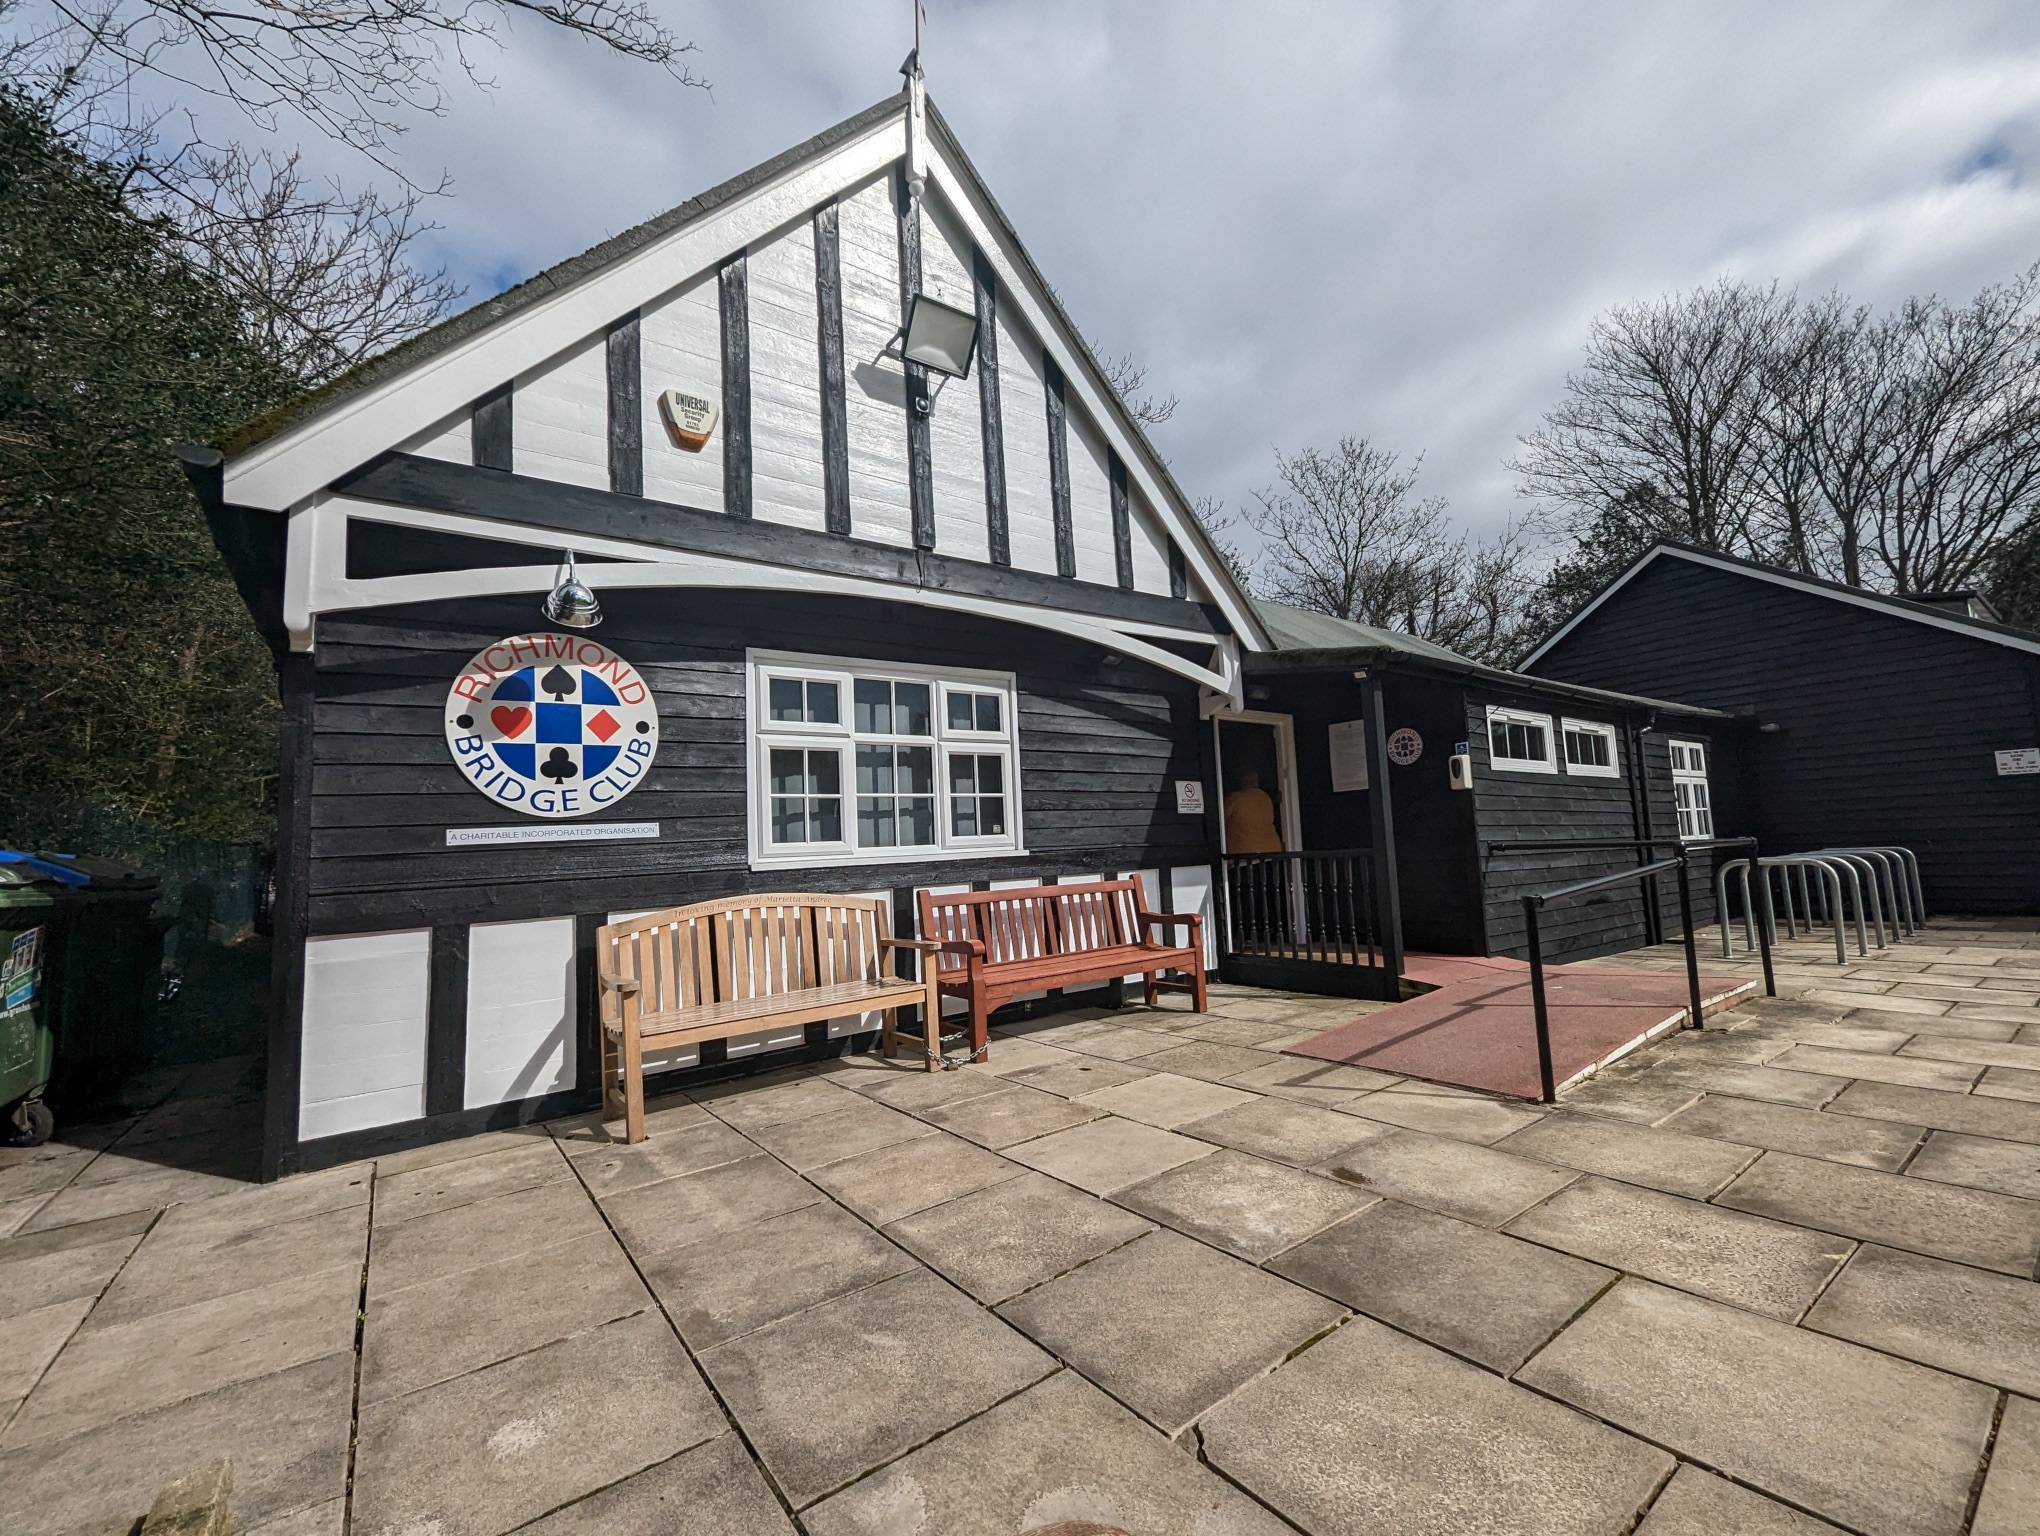
\includegraphics[width=6cm]{tournament1}
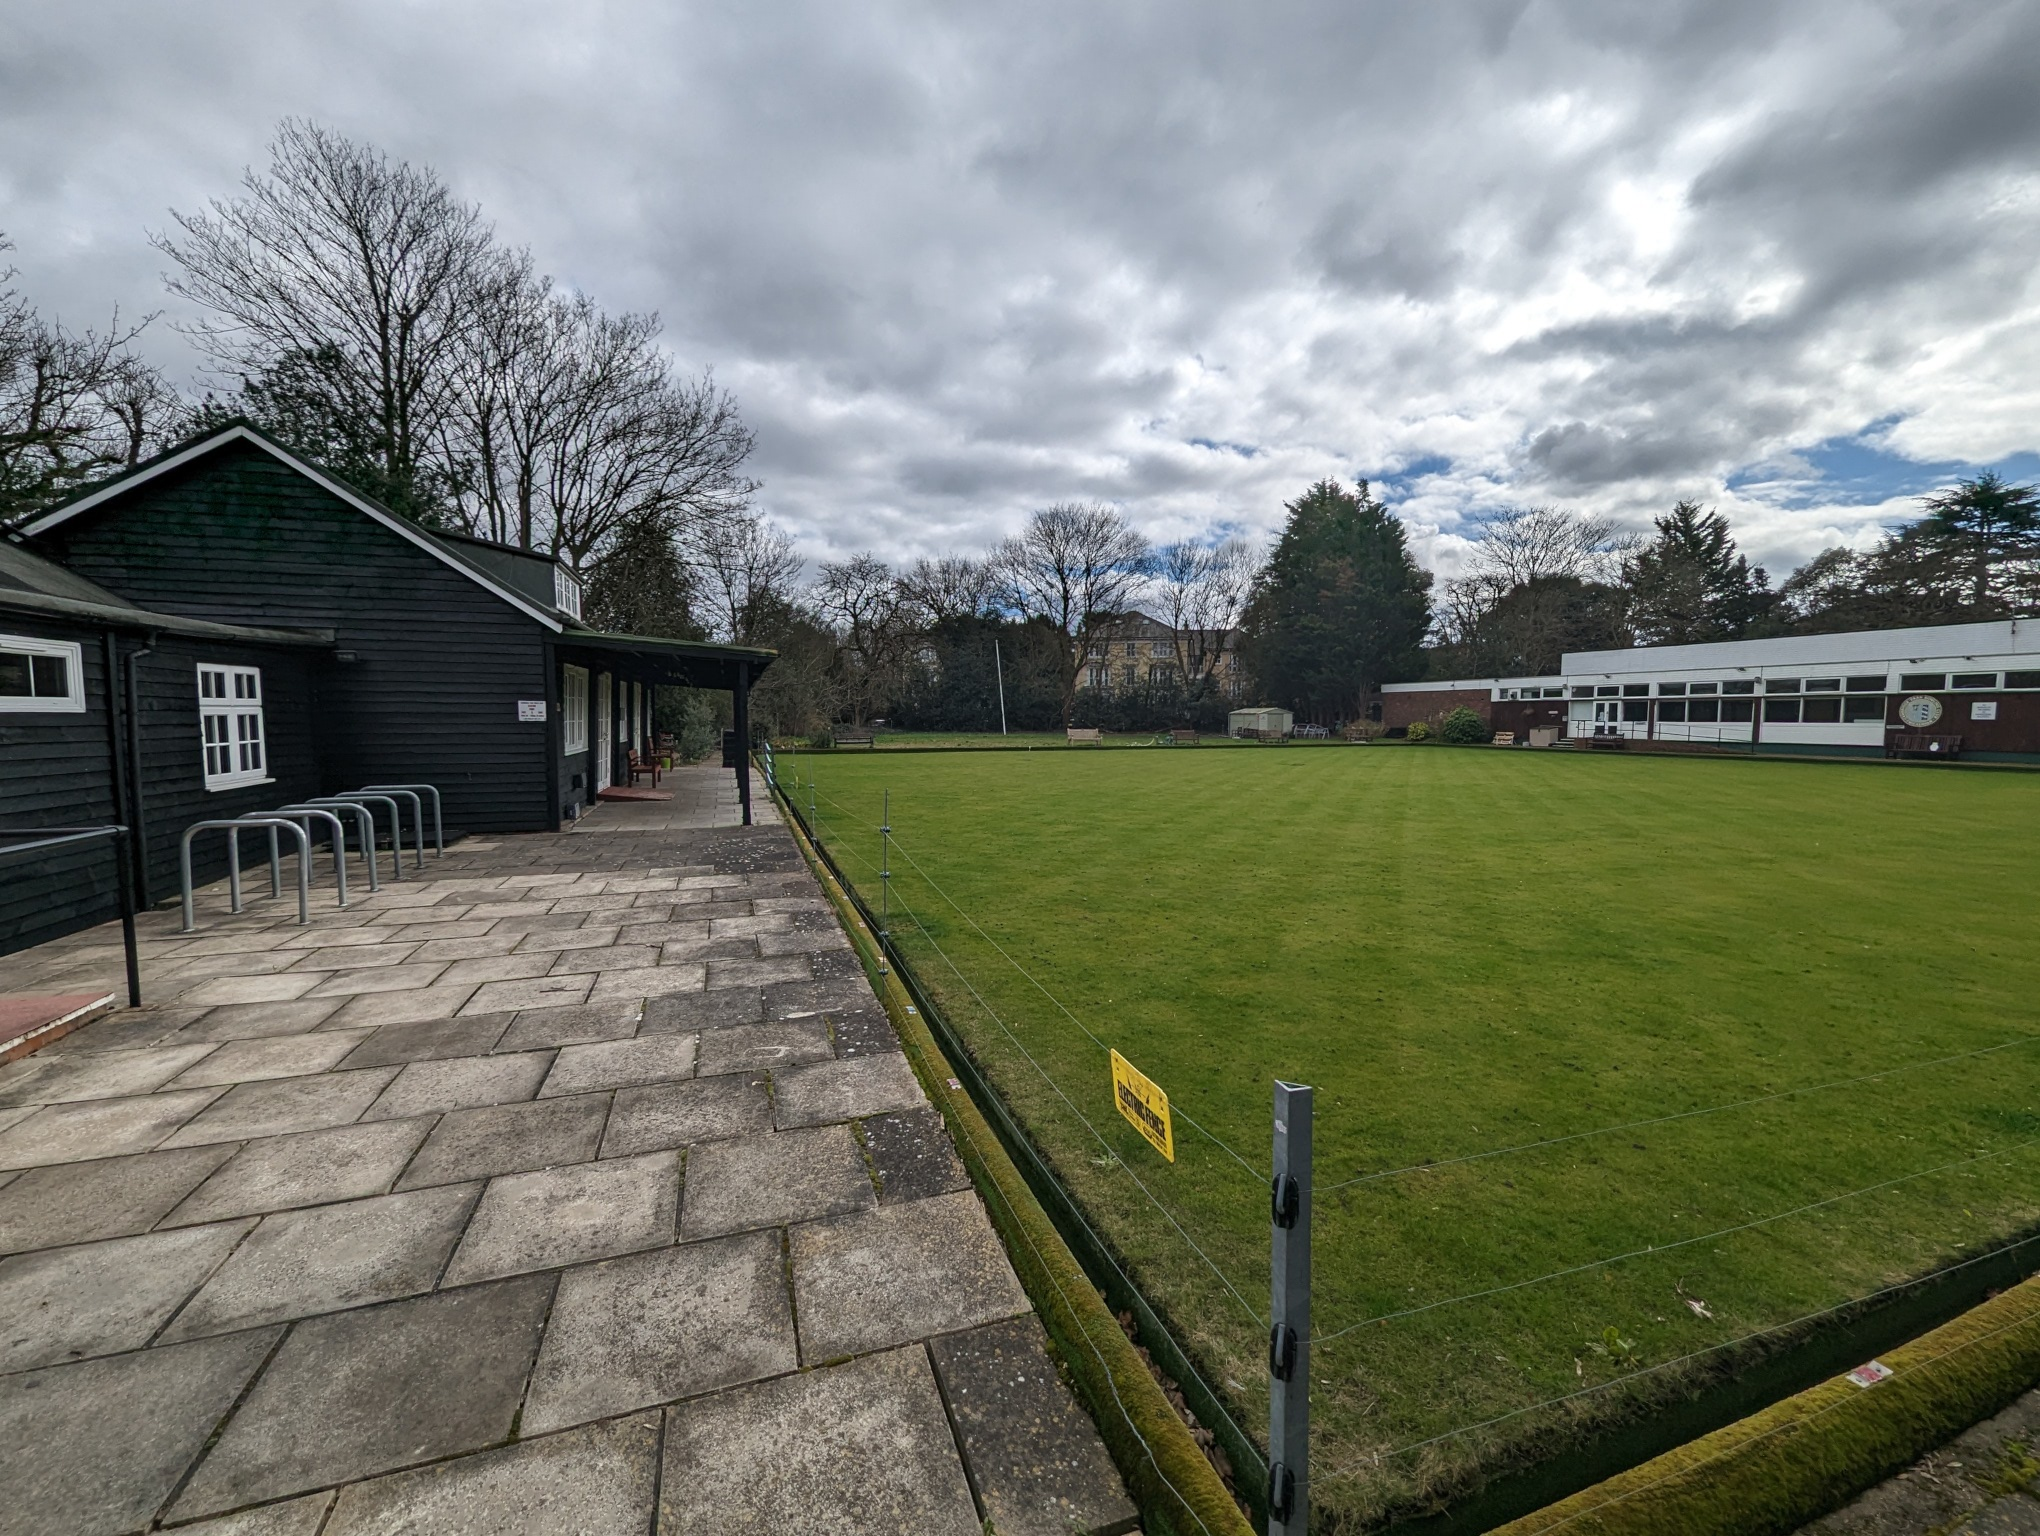
\includegraphics[width=6cm]{tournament2}
\end{figure}

\repsec{Equipment}
We played with good-quality mahjong sets and tables.

\repsec{Refereeing}
Two playing referees.

\repsec{Complaints}
None.

\repsec{Information/communication during the tournament}
A well-visible clock is projected from a computer on multiple screens placed around the tournament room.
A gong clearly informs players of the start and the end of sessions.
Up-to-date ranking between each session is displayed on the monitors.
A website with up-to-date ranking publicly available.

\repsec{Sessions}
Excellent playing atmosphere, FFF (Fair-play, Friendly, and Fun).

\begin{figure}[ht]
\centering
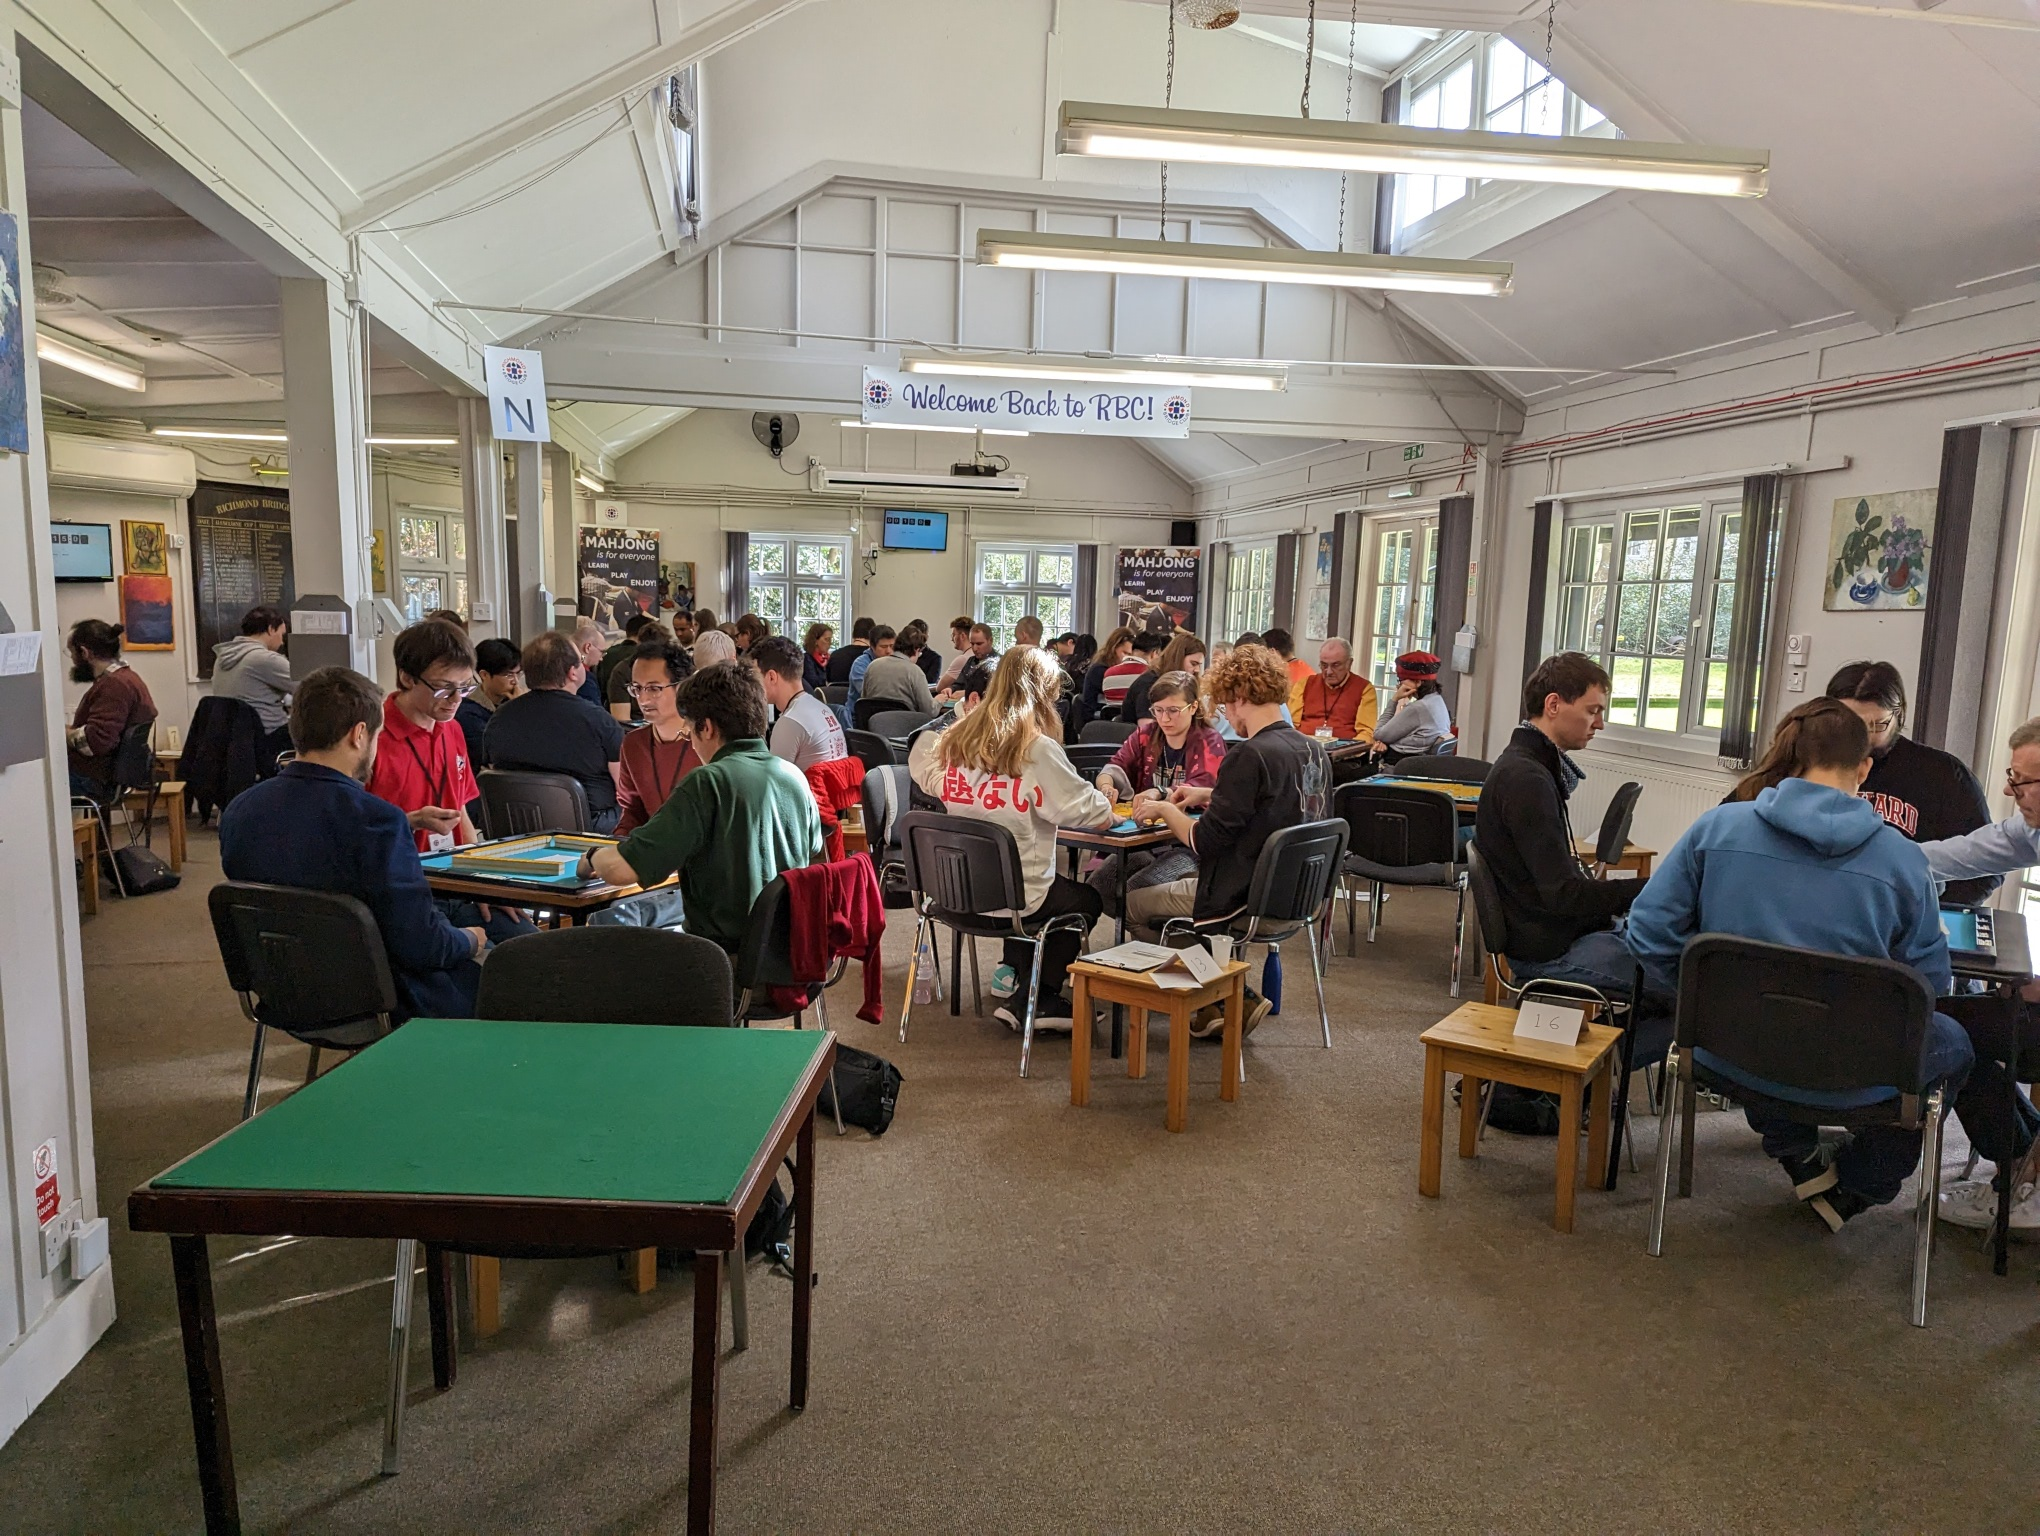
\includegraphics[width=8cm]{tournament3}
\end{figure}

\repsec{Catering}
Lunch in the same place, tea and coffee available.
Other drinks (including alcoholic ones) are available to buy at the venue.
Optional afterparty dinner on Saturday in a restaurant nearby.

\repsec{Prizes}
Trophies for individual ranking (1\textsuperscript{st}, 2\textsuperscript{nd} and 3\textsuperscript{rd}).

\repsec{Other comments}
\begin{itemize}
    \item It would be nice to have a full agenda on the reverse side of the player's badge.
    \item The organizers didn't wait for all the players to build the wall before starting a hanchan.
        However, I reported the issue and it was addressed in later games.
\end{itemize}

\repsec{Conclusion}
A well-organised tournament in Twickenham, good venue and a wonderful atmosphere.
All information was clearly provided.
Overall, this event is a success.

\end{document}
